\chapter{Implementation}

\section{Introduction}
Given the real-time nature of a CEP engine and the extensive uptime typical of a server, a thorough implementation is of maximum importance.

In this chapter I will explain how the project is structured and how it evolved in time, highlighting the choices made to find a balance between performance and convenience.

\section{Overview}
The TRex project, in its entirety, is composed of the engine library, a server, a client and an HTTP proxy. The engine, written in C++ and later in CUDA, is the foundation of the whole system and contains the business logic and the computationally intensive tasks. The server, written in C++ as well, links the core library and provides a network interface on top of it, receiving and dispatching packets for rules and events. The client, written in Java, allows full interaction with the CEP server via TCP/IP sockets: from publish-subscribe, to rule registration, using a TESLA parser created with ANTLR. The proxy, written in JavaScript for NodeJS, exposes an HTTP interface for publishing and subscribing, but at the moment doesn't implement rule parsing and registration. For the purpose of the thesis we will focus on the library, since its is the only one relevant in terms of feasibility and performance of static data integration.

At the beginning of the collaboration the TRex engine was a reasonably complex and well performing piece of software, although it showed several signs of its age. It was crafted over different iterations starting from 2010 and at that time C++ was still shaped according to its 12 years old original standardization. The very next year the C++11 standard came along, beginning an incredible period of renovation for both the language and the libraries, and the adoption of these new paradigms could really improve safety and extensibility.\\
In particular the broad usage of dynamically allocated objects requires exceptional caution during refactoring, because any minimal oversight could lead to memory leaks or attempts to access freed memory. In TRex it was handled with manual reference counting, which is now replaceable by `shared_ptr<T>` that uses RAII to relieve the programmer from the responsibility of updating the count.\\
Similarly a big part of the execution relies on the combination of type unions, enums and switches to describe and process TESLA expressions. The access to the wrong type or the absence of a switch case can cause bugs that aren't detected by the compiler and lead to unexpected runtime failures. In the upcoming C++17 the type `variant` will be added to the standard library (but it's already available in independent implementations) and it uses the power of template metaprogramming to prevent those issues at compile time.\\
Moreover threading utilities and paradigms are continuously evolving and they offer new levels of abstraction that reduce the needs of synchronization and locking, improving performances and preventing data races and deadlocks.\\
In addition to those safety benefits, there are several small improvements in terms of comprehensibility: like replacing array pointers with vectors, avoiding output arguments now that compilers handle efficiently the return statement, abandoning the cumbersome naming (inherited from the C tradition) for a wise usage of namespaces, adopting foreach loops and making use of idiomatic std functions.

Initially, when I started looking component by component to get familiar with the codebase, I tried to refactor where possible. The results were interesting in terms of simplification and had no significant performance lost, but the method was slow: it needed a lot of care, extensive testing and code reviews. After a while I noticed that I was only scratching the surface and further improvements implied huge changes across the whole repository. The task seemed so overwhelming that I started thinking about a complete rewrite.\\
The idea surely looked appealing and offered the opportunity to take only the best from years of experience, but it was extremely risky. Unable to choose, I kept cleaning and extending the old core and at the same I made some attempts to rethink the interfaces, I started experimenting with the different `variant` libraries and I even dived into the obscure albeit fascinating topic of template metaprogramming, in the hope of speeding up the development process.\\
Finally I reached a turning point, I got stuck with the extension of TRex and every modification seemed to be inconclusive, so I gave the rewrite I real chance, but instead of using the aforementioned C++ libraries I decided to use Rust, a new language which offers the same advantages and even more. 

\section{Rust}
Rust was born around 2010 as a side project of a Mozilla engineer and later backed by the company. The first pre-alpha release was reached in 2012 and the project hit version 1.0 in May 2015. So the language is pretty young and still missing some of its planned features, but many signs suggest that it may be on the right path.\\
First of all, while in the past there were several radical changes, after they reached the release 1.0 they committed to stability and backward compatibility, adopting a well defined workflow based on reference proposals. However the project has kept evolving quickly, with a release train model over 3 months windows.\\
Moreover it has raised a lot of interest within the community and there is a strong traction from a big company, ensuring continuity. Finally it is already used in production by Mozilla itself, Dropbox and Coursera among the others.

Rust aims to be a safe and practical language for system programming, with particular attention to concurrency. Its syntax, modern and expressive, combines the best aspects of imperative, object oriented and functional programming, offering the right level of abstraction for many different task.\\
The type-system, inspired by Haskell, is based on the concept of trait, which describe a property or a behavior of an object. Traits achieve their maximum utility in combination with generics, allowing code reuse while imposing clear restrictions on the applied types.\\
Rust also implements some features typical of higher level languages, like advanced union types (enums in Rust jargon), tuples, type inference, destructuring and pattern matching.\\
However the most prominent and peculiar characteristic is its unprecedented approach to safety with the concept of data ownership. Each object is tied to a single owner at a time, ownership can be transferred via assignment, return or function arguments and the content is moved and no longer accessible from the previous variable. If we want to access data without loosing ownership, it's possible to borrow multiple immutable references or a single mutable one, in the meantime the variable is considered blocked in something conceptually similar to a read-write lock. Every reference is bounded by the lifetime of the referee and can't outlive the owner. In this way is always clear who is responsible for the resource and when the owner goes out of scope the object can be safely dropped.\\
All these constraints and other minor ones are statically checked by the compiler, which gives strong guarantees of memory safety with no runtime overhead.

\begin{minipage}{\textwidth}
\begin{lstlisting}[caption={Example of borrow},label={lst:borrow},xleftmargin=.2\textwidth]
fn main() {
  // `a` is the owner of `3`
  let a = 3;

  // Beginning of a scoped block
  {
    // `a` is immutably borrowed by `b`
    let b = &a;
    // `a` is borrowed again by `c`
    let c = &a;
    assert!(*b == *c)

    // `a` can't be mutably borrowed
    // This would fail to compile
    let d = &mut a;

    // End of borrows
  }

  // Here is ok to mutably borrow
  let e = &mut a;

  // End of borrow
  // End of `a` scope, `3` dropped
}
\end{lstlisting}
\end{minipage}\\

Last but not least it worth mentioning that there is a growing ecosystem of tools and utilities, that ease setup and development. For example: rustup.rs is an automated setup and update script, cargo is a modern and simple package manager, build tool and documentation generator, crates.io is the official repository of open source libraries, rustfmt is a customizable code beautifier and racer is a code completion utility. It's also thanks to this simplicity of bootstrap and distribution, that I was persuaded to adopt this new technology.

\section{Architecture}
The TRex rewrite is composed by three crates (Rust jargon for packages): tesla, that contains basic engine interfaces and language structures, trex, that is the implementation of those traits, and benches,  a set of executables to test performances under simulated workload (on which we will focus in next chapter).

\subsection{Tesla}

\begin{figure}[h]
  \centering
  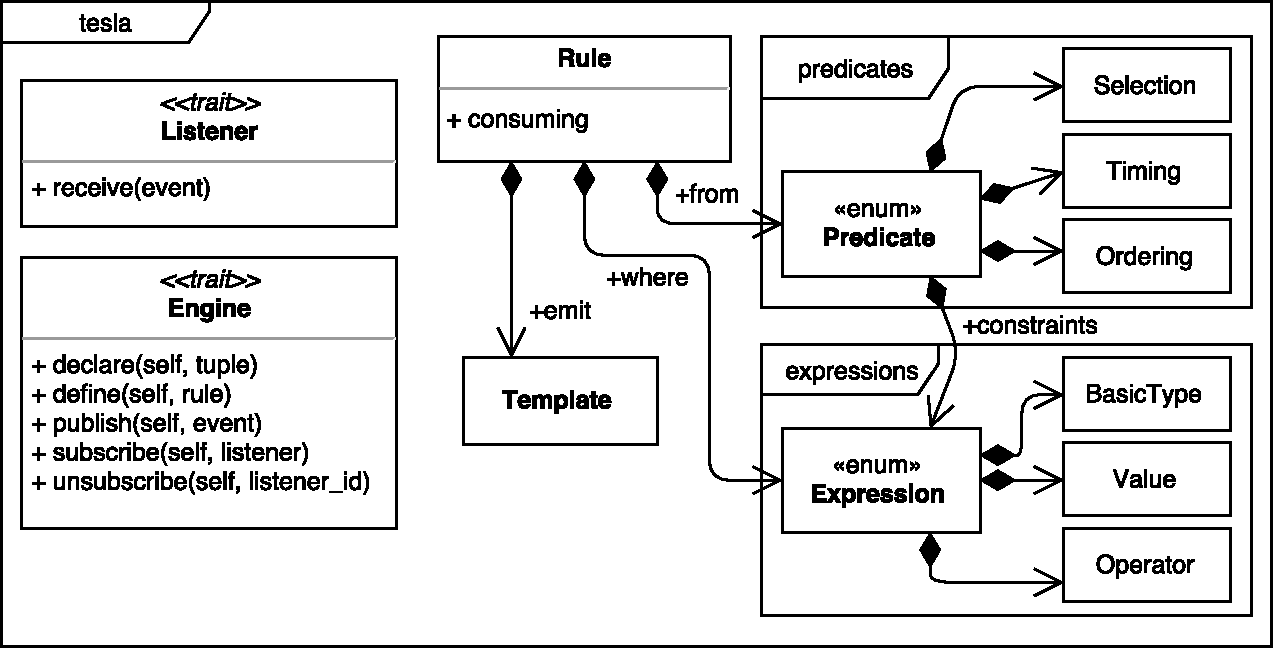
\includegraphics[width=\textwidth]{tesla_classes}
  \caption{Tesla crate overview}
\end{figure}

In tesla package I extracted all the aspects that aren't implementation related, so that it could work as minimal contact point between components like library and server. The core of the package is made of two traits: `Engine`, that defines methods for publish-subscribe, tuple declaration and rule definition, and `Subscriber`, that is used for event reception. Starting from these entry points the rest of the data structures just follows from the the information required: in particular we have two sub-packages `predicates` and `expressions`, the first contains all the tools to describe patterns of events and static data, the latter contains the AST of algebraic and comparison expressions. They both heavily leverage rust native union type, giving them a terse design compared to the possible equivalent with C++ `variant`.

\subsection{TRex}

\begin{figure}[h]
  \centering
  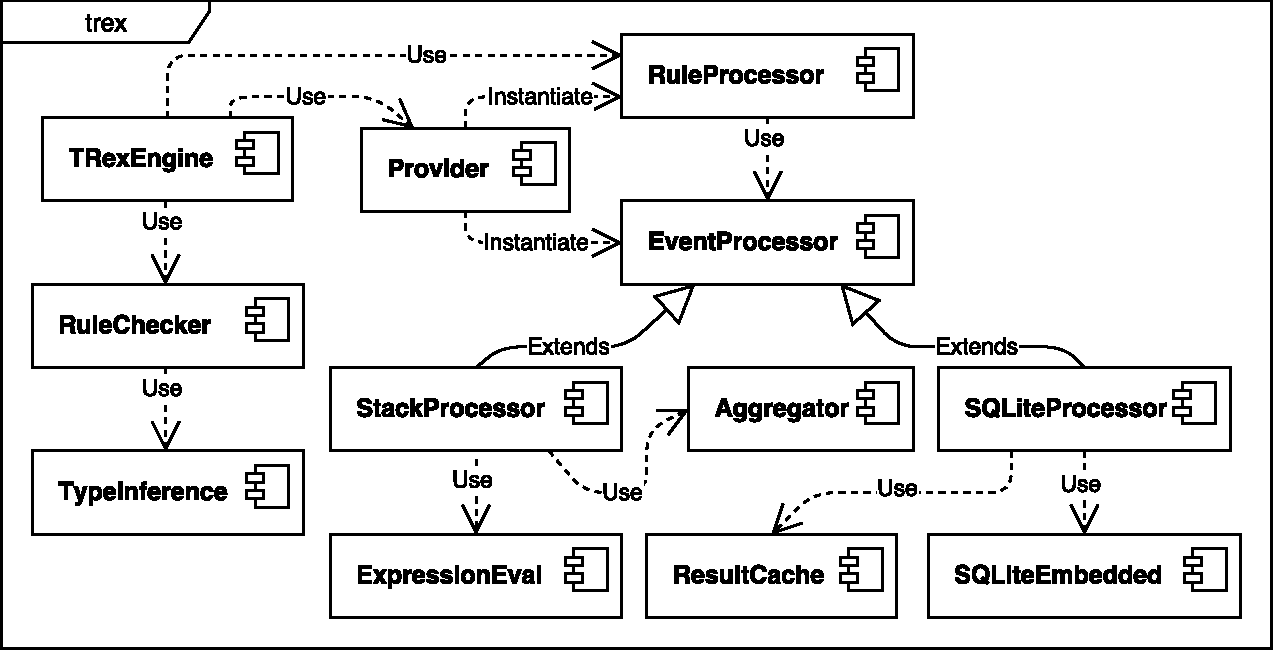
\includegraphics[width=\textwidth]{trex_components}
  \caption{TRex crate overview}
\end{figure}

The structure of `trex` crate closely recalls the previous implementation, with some simplification and new abstractions.

The core is the `TRex` struct, that implements the `Engine` trait and acts as a coordinator between the different components and the external world. When a new rule is defined `TRex` invokes the validation module and types, inferred using the previously collected tuple declarations, are checked to be used properly in expressions and assignments. If the rule satisfies the examination, the engine creates the dedicated processor using a factory pattern. The processor is indexed by events of interest and the system is ready to process incoming notifications. In the original project the index was more sophisticated than a single hash-map and had a mechanism to filter results with predicates static constraints. In practice the alternative appears to work well enough and additional optimization could be added if needed.

The most important changes are the ones concerning the event processing components. The rule processor, which corresponds to `StackRule` class in C++, is responsible of dispatching incoming event to the correct predicates and, in case of trigger activation, of propagating the chain of evaluation. In the previous version the different types of predicates were often coupled with business logic and in particular `StackRule` had to handle all of them explicitly, with specific functions and separate collections. In the rewrite there is the trait `EventProcessor` which is implemented by any component that is going to act as a predicate evaluator. In this way everything is handled uniformly: event processors are instantiated through a provider and packed in a single collection, every time that a notification arrives all the elements of the list is notified and each of them decide how to handle the information. When a trigger event arrives, an evaluation chain is started and it propagate between subsequent predicates in form of `PartialResults`.\\
This design choice makes it much easier to experiment with new data sources and hopefully this modularity will facilitate future development of custom components for different DBMS.

Currently the system runs two components: `StackProcessor`, which supports previous functionalities, and `SQLiteProcessor`, that is the test implementation of interoperability with a relational DB.\\
The `StackProcessor` implements CDP algorithm and, after verifying that every static constraints is satisfied, stores incoming event in a time ordered vector, which is periodically cleaned from old or consumed entries. When the evaluation starts and a `PartialResult` is received, the processor scans the events and propagates those that match every parameterized constraint.\\
The `SQLiteProcessor`, instead, doesn't interact with event notifications and it's activated only during the evaluation phase, when it queries the database to find suitable tuples.

\section{SQLite module}
The SQLite module contains two main components: a translator and an executor.

At creation time the predicate is fed to the translator and TESLA syntax is mapped permanently to a SQL statement using the following simple conversion rules.\\
The basic example is composed of an each predicate with no constraints nor parameters and, as we can see, the statement can be translated to a simple SQL select.
\begin{align*}% Example of each
&each\ SD\ \triangleq\\
&SELECT\ 1\ FROM\ SD;
\end{align*}
When the predicate features a negation, the operator `NOT EXIST` can be used to evaluate a subquery and return whether there are values in the result set or not.
\begin{align*}% Example of not
&not\ SD\ \triangleq\\
&SELECT\ NOT\ EXIST\ (SELECT\ 1\ FROM\ SD);
% For unexpected speed difference consider also:
% SELECT (SELECT id FROM SD) IS NULL;
% SELECT id FROM SD LIMIT 1;
\end{align*}
The selection policy $first$ does not have an implicit absolute ordering to work with, so it has to define one. The order clause is directly mapped to the SQL one.
\begin{align*}% Example of first
&first\ SD\ order\ by\ attr_1\ ASC,\ \ldots,\ attr_n\ DESC\ \triangleq\\
&SELECT\ id\ FROM\ SD\\
&ORDER\ BY\ attr_1\ ASC,\ \ldots,\ attr_n\ DESC\ LIMIT\ 1;
\end{align*}
For $last$ the same considerations made for $first$ hold, except for the mapping of the order clause, which is inverted.
\begin{align*}% Example of last
&last\ SD\ order\ by\ attr_1\ ASC,\ \ldots,\ attr_n\ DESC\ \triangleq\\
&SELECT\ id\ FROM\ SD\\
&ORDER\ BY\ attr_1\ DESC,\ \ldots,\ attr_n\ ASC\ LIMIT\ 1;
\end{align*}
The use of constraints inside tuple brackets find its correspondence in the SQL where clause.
\begin{align*}% Example of attribute constraint
&each\ SD(attr_1\ op \ val_1,\ \ldots,\ attr_n\ op \ val_n)\ \triangleq\\
&SELECT\ id\ FROM\ SD\\
&WHERE\ attr_1\ op\ val_1\ AND\ \ldots\ AND\ attr_n\ op\ val_n;
\end{align*}
The definition of a parameter it's processed adding its value to the query return column.
\begin{align*}% Example of parameter
&each\ SD[\$param = attr_i,\ \ldots]\ \triangleq\\
&SELECT\ attr_i\ as\ param,\ \ldots\ FROM\ SD;
\end{align*}
Finally the most common aggregation functions can be found in both the languages, so a translation is immediate.
\begin{align*}% Example of aggregates
&\$param\ =\ AGGR(SD.attr_1)\ \triangleq\\
&SELECT\ AGGR(attr_1)\ as\ param\ FROM\ SD
\end{align*}
The prepared statement produced is then stored for later use.

When the evaluation start, the executor populates the query with the parameters contained in `PartialResult` and execute it through `rusqulite` library (that is a wrapper of C SQLite embedded API) and the result are processed and forwarded in the chain of execution.

\section{Cache}
To improve performance of data retrieval and try to keep the speed of execution above the constraints of real-time, a caching layer was added between the executor and the database.\\
The key of the cache is made by the combination of a statement and the parameters with which it was populated. The key is intuitively unique for each result set\footnote{For the purpose of the thesis the data are considered immutable and cache invalidation is omitted} and it is also descriptive of the interrogation itself. So, instead of contacting the database directly, the executor will prepare a key and pass it to a fetcher. This new component will attempt a lookup in the cache table and if the result is a miss will fall back to the DB, hiding the complexity of cache update and multi-threaded synchronization.

The system is integrated with several cache algorithms that can be activated and configured through the engine construction arguments.\\
First of all there is a dummy cache that doesn't store anything and it's useful for testing the purposes in condition of 100\% misses.\\
Then there is a simple collision cache, that is an hashmap with a reduced key space and the insertion possibly removes an entry with the same hash value.\\
More interesting is the well known LRU, whose update function keeps track of the order of access and prioritize time locality. However, results sets can vary significantly in length, in contrast with the need of keeping a controlled memory footprint, so a variant called LRU-size was introduced. LRU-size has a maximum capacity set in terms of object sizes and, every time a value is inserted, multiple entries can be evicted to make room for the new one.\\
\begin{minipage}{\textwidth}
\begin{lstlisting}[caption={LRU-size insertion},label={lst:lrusize},xleftmargin=.15\textwidth]
function insert(key, entry) :=
  while memory usage + entry size > capacity
    remove least recent used entry
  done
  store entry as most recently used
end
\end{lstlisting}
\end{minipage}\\
\\
Finally, in the attempt of better exploiting heterogeneous data size and cost of retrieval, I implemented Greedy-Dual Size Frequency (GDSF) algorithm \cite{gdsf}, that is used by web browsers and, for example, by Squid caching proxy.\\
GDSF compute priority as a combination of how costly it is to obtain the entry, the size it occupies and the frequency it was accessed so far, with the following formula:
\begin{align*}
priority\ :=\ cost\ *\ frequency\ /\ size\ +\ clock
\end{align*}
Where $clock$ is an aging factor to avoid stagnation of entries that aren't relevant anymore and it's updated monotonically as the priority value of the last discarded entry.
